%!TEX root = ../template.tex
%%%%%%%%%%%%%%%%%%%%%%%%%%%%%%%%%%%%%%%%%%%%%%%%%%%%%%%%%%%%%%%%%%%%
%% chapter2.tex
%% NOVA thesis document file
%%
%% Chapter with the template manual
%%%%%%%%%%%%%%%%%%%%%%%%%%%%%%%%%%%%%%%%%%%%%%%%%%%%%%%%%%%%%%%%%%%%

\typeout{NT FILE demmon.tex}

\chapter{DeMMON}
\label{cha:demmon}

DeMMon (Decentralized Management and Monitoring Overlay Network) is an overlay network aiming to create logical connections among nodes integrating the network, forming multiple tree-shaped networks. Then, it provides an API to request information about nodes and services running in the system, which is collected on-demand by the monitoring protocol via efficient information aggregation and dissemination using the tree structure.

In this chapter, we will begin by explaining the targeted environment and the operation of the overlay network, whose tree shape is the basis for the aggregation protocol. After, detail how the aggregation protocol performs aggregations in the tree, and lastly, list the operations exposed by the API and discuss how it interacts with the remaining components. \todo{insert refs to subsections ahead}

This solution, as observable in figure \ref{fig:demmon-overview}, is composed of three major components:

\begin{figure}[htbp]
    \centering
    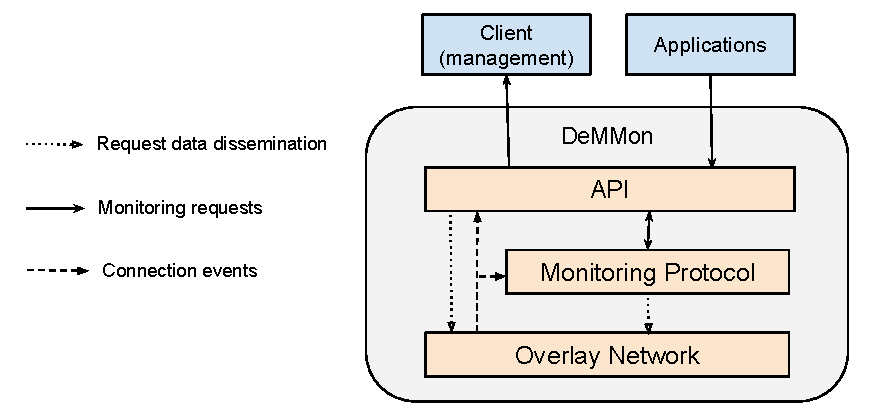
\includegraphics[width=\textwidth]{Chapters/Figures/DeMMon-arch-overview.pdf}
    \caption{An overview of the architecture of DeMMon}
    \label{fig:demmon-overview}
\end{figure}


\begin{enumerate}
    \item The overlay network, which strives to build the tree-shaped network, nodes in this network use proximity and a set of logical rules to change their location in the tree.

    \item The monitoring protocol, which is a component that collects and disseminates information using the overlay network's established connections. It communicates via notifications and asynchronous request-replies with the overlay network to receive updates regarding established connections and connection failures. Lastly, it receives requests from the API to collect information.

    \item Lastly, the API receives updates from both the overlay network and the monitoring protocol, exposes the received information from those layers, and allows ingestion of new information. Furthermore, it allows issuing commands to collect new information, perform local aggregations periodically, or trigger issued alarms based on the respective conditions.
\end{enumerate}

\section{Overlay network}

In this section, we discuss the design of the overlay network, which aims to build and maintain a latency and bandwidth aware tree-shaped network. We begin by providing the considered system model, then follow with an overview of the mechanisms responsible for building and maintaining the tree. Lastly, we conclude the chapter with a summary and discussion of the protocol.

\subsection{System Model}

The assumed system model is a distributed scenario composed of nodes connected to the internet set-up such that they can send and receive messages via the internet (i.e. with an external IP or port-forwarding). All nodes are running the GO-Babel framework with the same configuration settings, and that each node knows a priori a set of nodes to join the network (also denoted by landmarks). Optionally, the protocol can employ bandwidths to impose additional constraints in the tree-building procedures, so nodes with higher bandwidths tend to be used at the top of the tree topology. In this case, the system administrator must also configure nodes with a heuristic of their bandwidth capacity. Lastly, every node must share the same configurations concerning the membership protocols' parameters, listed in the following subsection.  \todo {say nodes are bandwidth-constrained}

\subsection{Tree construction and maintenance}

The devised membership protocol is coalesced by five main mechanisms: (1) the \textbf{join} mechanism, which aims to establish the initial tree structure, (2) \textbf{active view maintenance} is the mechanism responsible for periodically sharing some state with peers, which later useful for tree optimizations, (3) \textbf{group optimization}, where nodes periodically attempt to optimize their childrens' active connections, (4) \textbf{passive view maintenance}, responsible for collecting information about peers which are not in the active view, used for fault tolerance and optimizations, and finally, (5) \textbf{oportunistic optimization}, where nodes may attempt to improve their position in the overlay based on latency and bandwidth. We will now cover each mechanism in the provided order.

As previously mentioned, the join mechanism is the mechanism responsible for creating the initial tree structure, it is the first mechanism to be executed by each node in the system, 

% JOIN -----

% Types :

% Node {
%     ID // string attributed by parent \asdupon[entering the syst]m
%     measuredLatency // the measured latency to the peer
%     parentIP // the IP of the parent of the Node
%     nrChildren // the number of children
%     replied // wether the node replied to joinMessage
%     IP // the node IP
%     children: [] {
%         ID  // the children id of the peer
%         nrChildren  // the nr of children of the child
%         IP // the node IP
%     }
% }

% Define tab size for indentation
\algrenewcommand\algorithmicindent{2em}%

%%%%%%%%%%%%%%%%%%%%%%%%%%%%%%%%%%%%%%%%%%%%%%%%%%%%%%%%%%%%%%%%
% BLOCKS - \block[]
%%%%%%%%%%%%%%%%%%%%%%%%%%%%%%%%%%%%%%%%%%%%%%%%%%%%%%%%%%%%%%%%

% State, like all blocks ends with \asdend
\algblockdefx[asdstate]{asdstate}{asdend}
{\textbf{State}}{}


% Init
\algblockdefx[asdinit]{asdinit}{asdend}
{\textbf{Init}}{}

\algblockdefx[asdtypes]{asdtypes}{asdend}
{\textbf{Types}}{}

\algdef{SE}[SUBALG]{Indent}{EndIndent}{}{\algorithmicend\ }%
\algtext*{Indent}
\algtext*{EndIndent}

% Upon
\algblockdefx[asdupon]{asdupon}{asdend}
[1][Unknown]{\textbf{Upon} #1 \textbf{Do}}{}
\algblockdefx[asdupontimer]{asdupontimer}{asdend}
[1][Unknown]{\textbf{Upon Timer} #1 \textbf{Do}}{}

% For
\algblockdefx[asdfor]{asdfor}{asdend}
[1][Unknown]{\textbf{Forall} #1 \textbf{Do}}{}

\algblockdefx[asdrepeateveryx]{asdrepeateveryx}{asdend}
[1]{\textbf{Every} #1 \textbf{Do}}{}

% If
\algblockdefx[asdif]{asdif}{asdend}
[1][Unknown]{\textbf{If} (#1) \textbf{Then}}{}

% Else for If
\algcblockdefx[asdelsea]{asdif}{asdelsea}{asdend}
{\textbf{Else}}{}

% Else for Else If
\algcblockdefx[asdelseb]{asdelseif}{asdelseb}{asdend}
{\textbf{Else}}{}

% Else If
\algcblockdefx[asdelseif]{asdif}{asdelseif}{asdend}
[1][Unknown]{\textbf{Else If} (#1) \textbf{Then}}{}

% Interface
\algblockdefx[asdinterface]{asdinterface}{asdend}
{\textbf{Interface}}{}

% Requests
\algblockdefx[asdrequests]{asdrequests}{asdend}
{\textbf{Requests}}{}

% Indications
\algblockdefx[asdindications]{asdindications}{asdend}
{\textbf{Indications}}{}

% Procedure
\algblockdefx[asdprocedure]{asdprocedure}{asdend}
[1][Unknown]{\textbf{Procedure} #1}{}

% Forever
\algblockdefx[asdforever]{asdforever}{asdend}
{\textbf{Forever Do}}{}

%%%%%%%%%%%%%%%%%%%%%%%%%%%%%%%%%%%%%%%%%%%%%%%%%%%%%%%%%%%%%%%%
% STATEMENTS - \statement{} or \statement{}{}
%%%%%%%%%%%%%%%%%%%%%%%%%%%%%%%%%%%%%%%%%%%%%%%%%%%%%%%%%%%%%%%%

% Simple Statements
\newcommand{\asdstatement}[1]{\statenew{#1}}
\newcommand{\asdstatementbold}[1]{\statenew{\textbf{#1}}}

% Trigger
\newcommand{\asdtrigger}[1]{\statenew{\textbf{Trigger} #1}}

% Timer
\newcommand{\asdsetuptimer}[1]{\statenew{\textbf{Setup Timer} #1}}
\newcommand{\asdsetupptimer}[1]{\statenew{\textbf{Setup Periodic Timer} #1}}
\newcommand{\asdcanceltimer}[1]{\statenew{\textbf{Cancel Timer} #1}}

% Call
\newcommand{\asdcall}[1]{\statenew{\textbf{Call} #1}}

% Return - use [] due to xparse
\NewDocumentCommand{\asdreturn}{o}{
	\statenew{\textbf{Return}\IfValueT{#1}{ #1}}
}

% Comment (inline)
\makeatletter
\newcommand{\asdcomment}[1]{
	\parbox[t]{\dimexpr\linewidth-\ALG@thistlm-8em}{
		\strut
		//\space #1
		\strut
	}
}
\makeatother


% Comment (entire line)
\makeatletter
\newcommand{\asdlinecomment}[1]{
		\State \parbox[]{\dimexpr\textwidth-\leftmargin-\labelsep-\labelwidth}{
			//\space #1
		\strut}
}
\makeatother


%%%%%%%%%%%%%%%%%%%%%%%%%%%%%%%%%%%%%%%%%%%%%%%%%%%%%%%%%%%%%%%%
% VALUES
%%%%%%%%%%%%%%%%%%%%%%%%%%%%%%%%%%%%%%%%%%%%%%%%%%%%%%%%%%%%%%%%

% Booleans
\newcommand{\asdfalse}[0]{$false$}
\newcommand{\asdtrue}[0]{$true$}

% Map
\newcommand{\asdmap}[2]{#1{[}#2{]}}

% Set 
\newcommand{\asdset}[1]{$\{$#1$\}$}

%%%%%%%%%%%%%%%%%%%%%%%%%%%%%%%%%%%%%%%%%%%%%%%%%%%%%%%%%%%%%%%%
% Algebraic
%%%%%%%%%%%%%%%%%%%%%%%%%%%%%%%%%%%%%%%%%%%%%%%%%%%%%%%%%%%%%%%%

% Equals (assignment)
\newcommand{\asdassign}[0]{ $\longleftarrow$ }

\algblockdefx[Foreach]{Foreach}{EndForeach}[1]{\For{\textbf{each} #1}}{}

% Equals (comparison)
\newcommand{\asdeq}[2]{#1 $=$ #2}

% Not equals
\newcommand{\asdneq}[2]{#1 $\neq$ #2}

% Exists
\newcommand{\asdexists}[1]{$\exists$ #1}

% Not Exists
\newcommand{\asdnexists}[1]{$\nexists$ #1}

% And
\newcommand{\asdand}[2]{#1 $\wedge$ #2}

% Or
\newcommand{\asdor}[2]{#1 $\vee$ #2}

% Except
\newcommand{\asdexcept}[2]{#1 $\setminus$ #2}

% Union
\newcommand{\asdunion}[2]{#1 $\bigcup$ #2}

% Belongs to
\newcommand{\asdin}[2]{#1 $\in$ #2}

% Not belongs to
\newcommand{\asdnotin}[2]{#1 $\notin$ #2}

% Bottom
\newcommand{\asdbottom}{$ \perp $}

\algnewcommand{\IfThenElse}[3]{% \IfThenElse{<if>}{<then>}{<else>}
  \State \algorithmicif\ #1\ \algorithmicthen\ #2\ \State \algorithmicelse\ #3}


%%%%%%%%%%%%%%%%%%%%%%%%%%%%%%%%%%%%%%%%%%%%%%%%%%%%%%%%%%%%%%%%
% Other
%%%%%%%%%%%%%%%%%%%%%%%%%%%%%%%%%%%%%%%%%%%%%%%%%%%%%%%%%%%%%%%%

\newcommand{\asdnewline}{\hfill\State}

\algblock[]{Start}{End}

\begin{algorithm}
\begin{algorithmic}[1]
    \caption{Join Protocol}
    \asdtypes
        \State Node \{
        \Indent
        \State     ID // string attributed by parent upon entering the system
        \State     measuredLatency // the measured latency to the peer
        \State     parentIP // the IP of the parent of the Node
        \State     nrChildren // the number of children
        \State     replied // wether the node replied to joinMessage
        \State     IP // the node IP
        \State     children: []<nrChildren,IP> 
        \EndIndent
        \State \}
    \asdend


    \asdstate
        \State minGroupSize // the minimum group size
        \State joinTimeouts // collection of timers for contacted nodes
        \State contactedNodes // map of all successfully contacted nodes
        \State nodesToContact // nodes being contacted
        \State bestPeerLastLevel // lowest latency peer in last level
        \State isLandmark // boolean indicating if peer is landmark peer
        \State joinTimeoutTimerID // timer id for join messages
        \State self Node // self
    \asdend

    \asdupon[Init(landmarkIps, selfIP)]
        \State joinTimeouts <- {}
        \State bestPeerLastLevel <- {}
        \State landmarks <- []
        \State isLandmark <- selfIP \asdin landmarkIps
        \asdif[isLandmark]
            \State progressToNextLevel(landmarkIps)
        \asdelsea 
            \asdfor[landmark in landmarks]
                \State dial(landmark)
            \asdend
        \asdend
    \asdend

    \asdupon[JoinTimeoutTimer(L)]
        \asdif (L in Landmarks)
        \State rejoinLater()
        \asdelsea
            \State delete(nodesToContact[L])
        \asdend
    \asdend

    \asdupon[JoinRequestTimeout(p)]
        \asdif[p.parentIP != nil]
        \State bestPeerLastLevel = contactedNodes[bestPeerLastLevel.parentIP]
        \State joinAsChild(bestPeerLastLevel)
        \asdelsea
            \State rejoinLater()
        \asdend
    \asdend

    \asdupon[receive(Join<>,sender)]
        \State cancelTimer(joinTimeouts[sender])
        \State delete(joinTimeouts, sender)
        \State sendMessageSideChannel(JoinReply<self.parent, self.node, self.children>, sender)
    \asdend

    \asdupon[receive JoinReply(<parentIP, node, children>, sender)]
        \State contactedNode = nodesToContact[node.IP]
        \State contactedNode.id = node.ID
        \State contactedNode.parentIP = parentIP
        \State contactedNode.nrChildren = len(children)
        \State contactedNode.replied = true
        \asdfor[c in children]
            \State contanctedNode.Children.append(\{ ID : c.ID, nrChildren <- c.nrChildren,
                IP <- c.IP
            \})
        \asdend
    \asdend

    \asdupon[receive(JoinRequestReply<>, sender)]
        \State // joined successfully! 
        \State // further assignments omitted
        \State addParent(sender)
    \asdend

    \asdupon[NodeMeasured(node, latency]
        \State nodesToContact[node].measuredLatency = latency
    \asdend

    \asdupon[NodeMeasuringFailed(node]{
        \State delete(nodesToContact, node)
    \asdend

    % \asdupon[forAll(n in nodesToContact -> n.measuredLatency != -1 && ].replied) {
    %     if len(nodesToContact) == 0 {
    %         if bestPeerLastLevel == nil { // has not gotten past landmarks
    %         rejoinLater()
    %         return
    %     }
    %     contactedNodes.appendAll(nodesToContact)
    %     for node in sortedByLatency(nodesToContact) {
    %         // check to see if parent's latency isn't lower than node's
    %         if bestPeerLastLevel != nil {
    %             if bestPeerLastLevel.measuredLatency < node.measuredLatency {
    %                 joinAsChild(bestPeerLastLevel)
    %                 return
    %             }
    %         }

    %         // check to see if node has enough children to become joiner's parent (unless its a landmark)
    %         if (node.IP not in landmarks) && node.nrChildren == 0  {
    %             continue
    %         }

    %         bestPeerLastLevel = node
    %         progressToNextLevel([c.IP for c in node.children])
    %         return
    %     }
    %     if bestPeerLastLevel.parentIP == nil {
    %         bestPeerLastLevel = contactedNodes[bestPeerLastLevel.parentIP]
    %         joinAsChild(bestPeerLastLevel)       
    %         return
    %     } else {
    %         rejoinLater()
    %     }
    % }

    % prodecude joinAsChild(p){
    %     joinTimeoutTimerID = setupTimer(JoinRequestTimeout<p>)
    %     sendMessageSideChannel(JoinRequest<>, p.IP)
    % }

    % prodecude progressToNextLevel(nodeIPs) {
    %     nodesToContact <- {}
    %     parentID <- nil
    %     if bestPeerLastLevel != nil { parentID <- bestPeerLastLevel.ID}

    %     for p in nodeIPs {
    %         nodesToContact[p] = Node {
    %             IP : p
    %             measuredLatency <- -1
    %             parentID <- parentID
    %             nrChildren <- -1
    %             replied <- false
    %             children <- []
    %         }
    %         sendMessageSideChannel(JoinMessage<>, p)
    %         t <- setupTimer(JoinTimeoutTimer{p})
    %         joinTimeouts[p] = t
    %         MeasureNode(p)
    %     }
    % }

\end{algorithmic}
\end{algorithm}

\subsection{Summary}

\section{Monitoring protocol}

\subsection{Overview}

\subsection{Aggregation mechanisms}

\subsubsection{Single root aggregation}

\subsubsection{Multi root aggregation}

\subsubsection{Neighborhood aggregation}

\subsection{Summary}

\section{API}

\subsection{System Model}

\subsection{Overview}

\subsection{Showcase}